\documentclass[color=blue, bottompic=3, uob, qetlabs, quantic, cdt, dstl]{uibkpost}
\usepackage{graphicx}
\usepackage[bookmarks=true, bookmarksnumbered=true, bookmarksopen=false, colorlinks=false, filecolor=black, linkbordercolor=blue, urlbordercolor=green, plainpages=false, pdfpagelabels, citebordercolor=uibkBlue, anchorcolor=red, pdfauthor=Stefan Frick, hyperfootnotes=false]{hyperref}
\usepackage[numbers, square, comma, sort&compress]{natbib}
\usepackage{amsmath}
\usepackage{amssymb}
\usepackage{amsfonts}
\usepackage{gensymb}
\usepackage{color}
\usepackage{braket}
\usepackage{comment}
\usepackage{mathtools}
\usepackage{siunitx}
\usepackage{import}
\usepackage{multirow}
\usepackage{setspace}
%\usepackage[dvipsnames]{xcolor}

\sisetup{
  mode = text,
  detect-family,
  detect-weight,
  color = uibkBlack}
\usepackage{pgfplots}
\pgfplotsset{compat=newest}
\usepgfplotslibrary{fillbetween}
\usepackage{tikz}
\usetikzlibrary{positioning}
\usetikzlibrary{calc}
\usetikzlibrary{arrows, shapes}
\usetikzlibrary{arrows.meta}
\usetikzlibrary{decorations.markings}
\usetikzlibrary{patterns}
\usetikzlibrary{backgrounds}


\renewcommand{\familydefault}{\sfdefault}
\renewcommand{\arraystretch}{1.5}
\graphicspath{{pics/}}



% package for diagonally divided cell in tables 
\usepackage{diagbox}

\bibliographystyle{stefan}

\title{Optimised parametric down-conversion sources for photonic quantum technologies} % Your article title
\author{\underline{T. Faleo}, C. L. Morrison, R. Beignon, F. Graffitti, V. Remesh, S. Frick, A. Fedrizzi, G. Weihs, R. Keil} % Your name
\date{\today} % Add a date here if you would like one to appear underneath the title block

%%%%%%%%%%%%%%%%%%%%%%%%%%%%%%%%%%%%%%%
% UOB COLOURS CORE PALETTE FOR LEGACY %
%%%%%%%%%%%%%%%%%%%%%%%%%%%%%%%%%%%%%%%
% (besides black and white)
\definecolor{uobRed}{RGB}{192,47,56}
\definecolor{uobStone}{RGB}{190,183,169}
%%%%%%%%%%%%%%%%%%%%%%%%%%%%%%
% COLOURS SUPPORTING PALETTE %
%%%%%%%%%%%%%%%%%%%%%%%%%%%%%%
\definecolor{uobBrightAqua}{RGB}{0,192,181}
\definecolor{uobDarkAqua}{RGB}{0,61,76}
\definecolor{uobBrightBlue}{RGB}{12,198,222}
\definecolor{uobDarkBlue}{RGB}{0,47,95}
\definecolor{uobBrightPurple}{RGB}{146,120,209}
\definecolor{uobDarkPurple}{RGB}{66,20,95}
\definecolor{uobBrightPink}{RGB}{224,36,154}
\definecolor{uobDarkPink}{RGB}{119,32,89}
\definecolor{uobBrightRed}{RGB}{224,0,52}
\definecolor{uobDarkRed}{RGB}{94,48,50}
\definecolor{uobBrightYellow}{RGB}{255,182,18}
\definecolor{uobDarkYellow}{RGB}{134,67,30}
\definecolor{uobBrightLime}{RGB}{190,214,0}
\definecolor{uobDarkLime}{RGB}{83,104,43}
\definecolor{uobBrightGreen}{RGB}{52,178,51}
\definecolor{uobDarkGreen}{RGB}{2,71,49}

\DeclareMathOperator{\SNR}{SNR}

%----------------------------------------------------------------------------------------
%	DOCUMENT
%----------------------------------------------------------------------------------------

\begin{document}

\begin{poster}
  \maketitle

  \abstract{
    Photonic quantum technologies rely on many-photon interference, necessitating the efficient generation of indistinguishable photons. Exceptional achievements have been obtained by nonlinear domain engineering of parametric down-conversion sources, with theoretical spectral purity up to 98.7\% and measured two-photon interference visibilities as high as 98.6(1.1)\% with loose spectral filtering [1]. 
    Here, we further optimise the purity of the down-conversion process by combining domain engineering and pump spectral shaping via a spatial light modulator (SLM) in a 4$f$ pulse shaper. This approach provides both a Gaussian quasi-phase-matching and a Gaussian pump envelope, enabling us to attain a measured spectral purity of 99.92(1)\% and a two-photon interference visibility of 98.5(1.5)\% without the necessity for spectral filtering.
  }

  \block{l}{Hong-Ou-Mandel interference and indistinguishability}{
    In photonic quantum technologies, the lack of direct photon interaction is compensated for by exploiting two-particle interference: the so-called Hong-Ou-Mandel (HOM) effect [2].
    This phenomenon occurs when two indistinguishable photons enter the input ports of a 50:50 beam splitter, manifesting in the suppression of coincidence events measured by the detectors. High visibility of this interference depends on achieving high indistinguishability in all internal degrees of freedom. These include relative delay (see figure below), polarisation, and frequency.\\[0.25cm]
    \raisebox{4ex}{
    \begin{minipage}[b]{0.5\textwidth}
        \begin{center}
            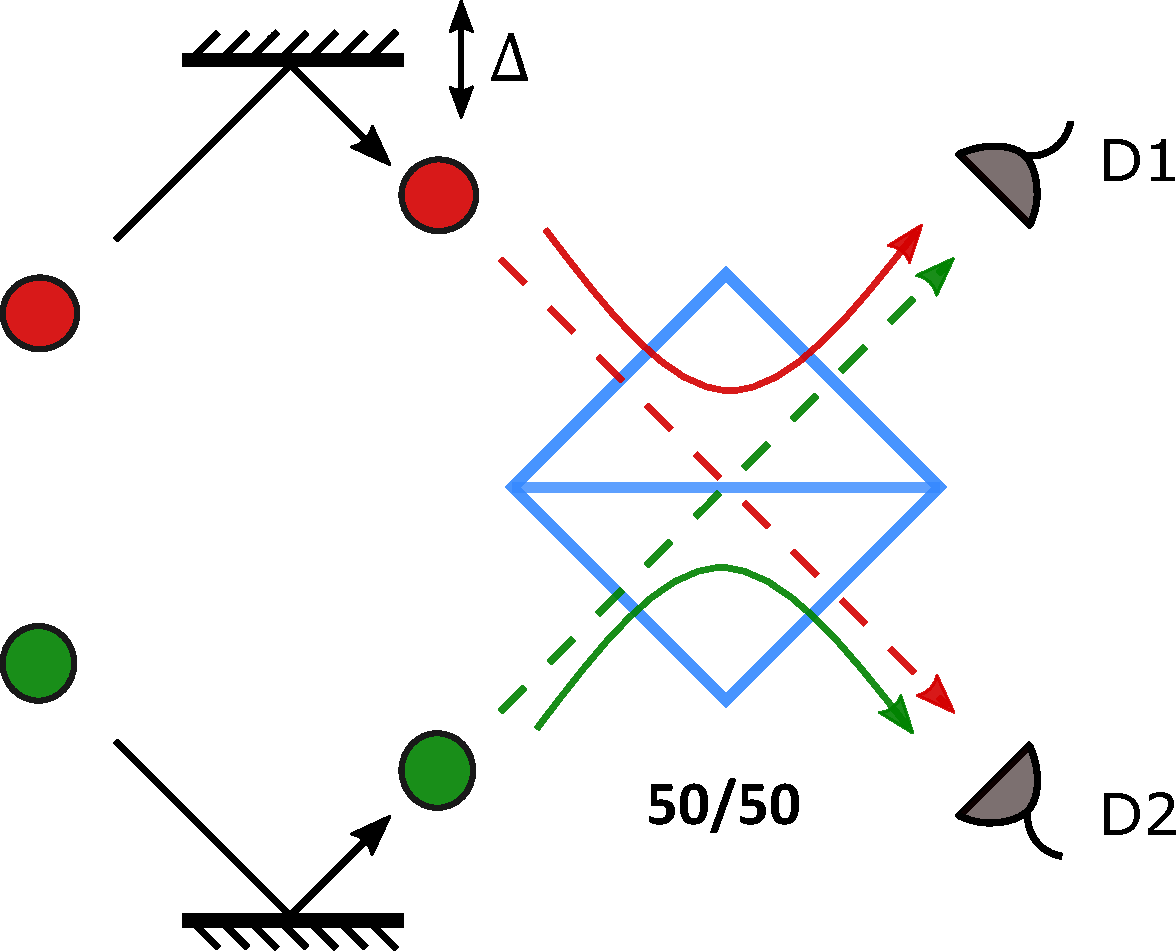
\includegraphics[width=0.6\textwidth]{pics/HOM_v3.pdf}
        \end{center}
    \end{minipage}}
    \begin{minipage}[b]{0.5\textwidth}
        \begin{center}
            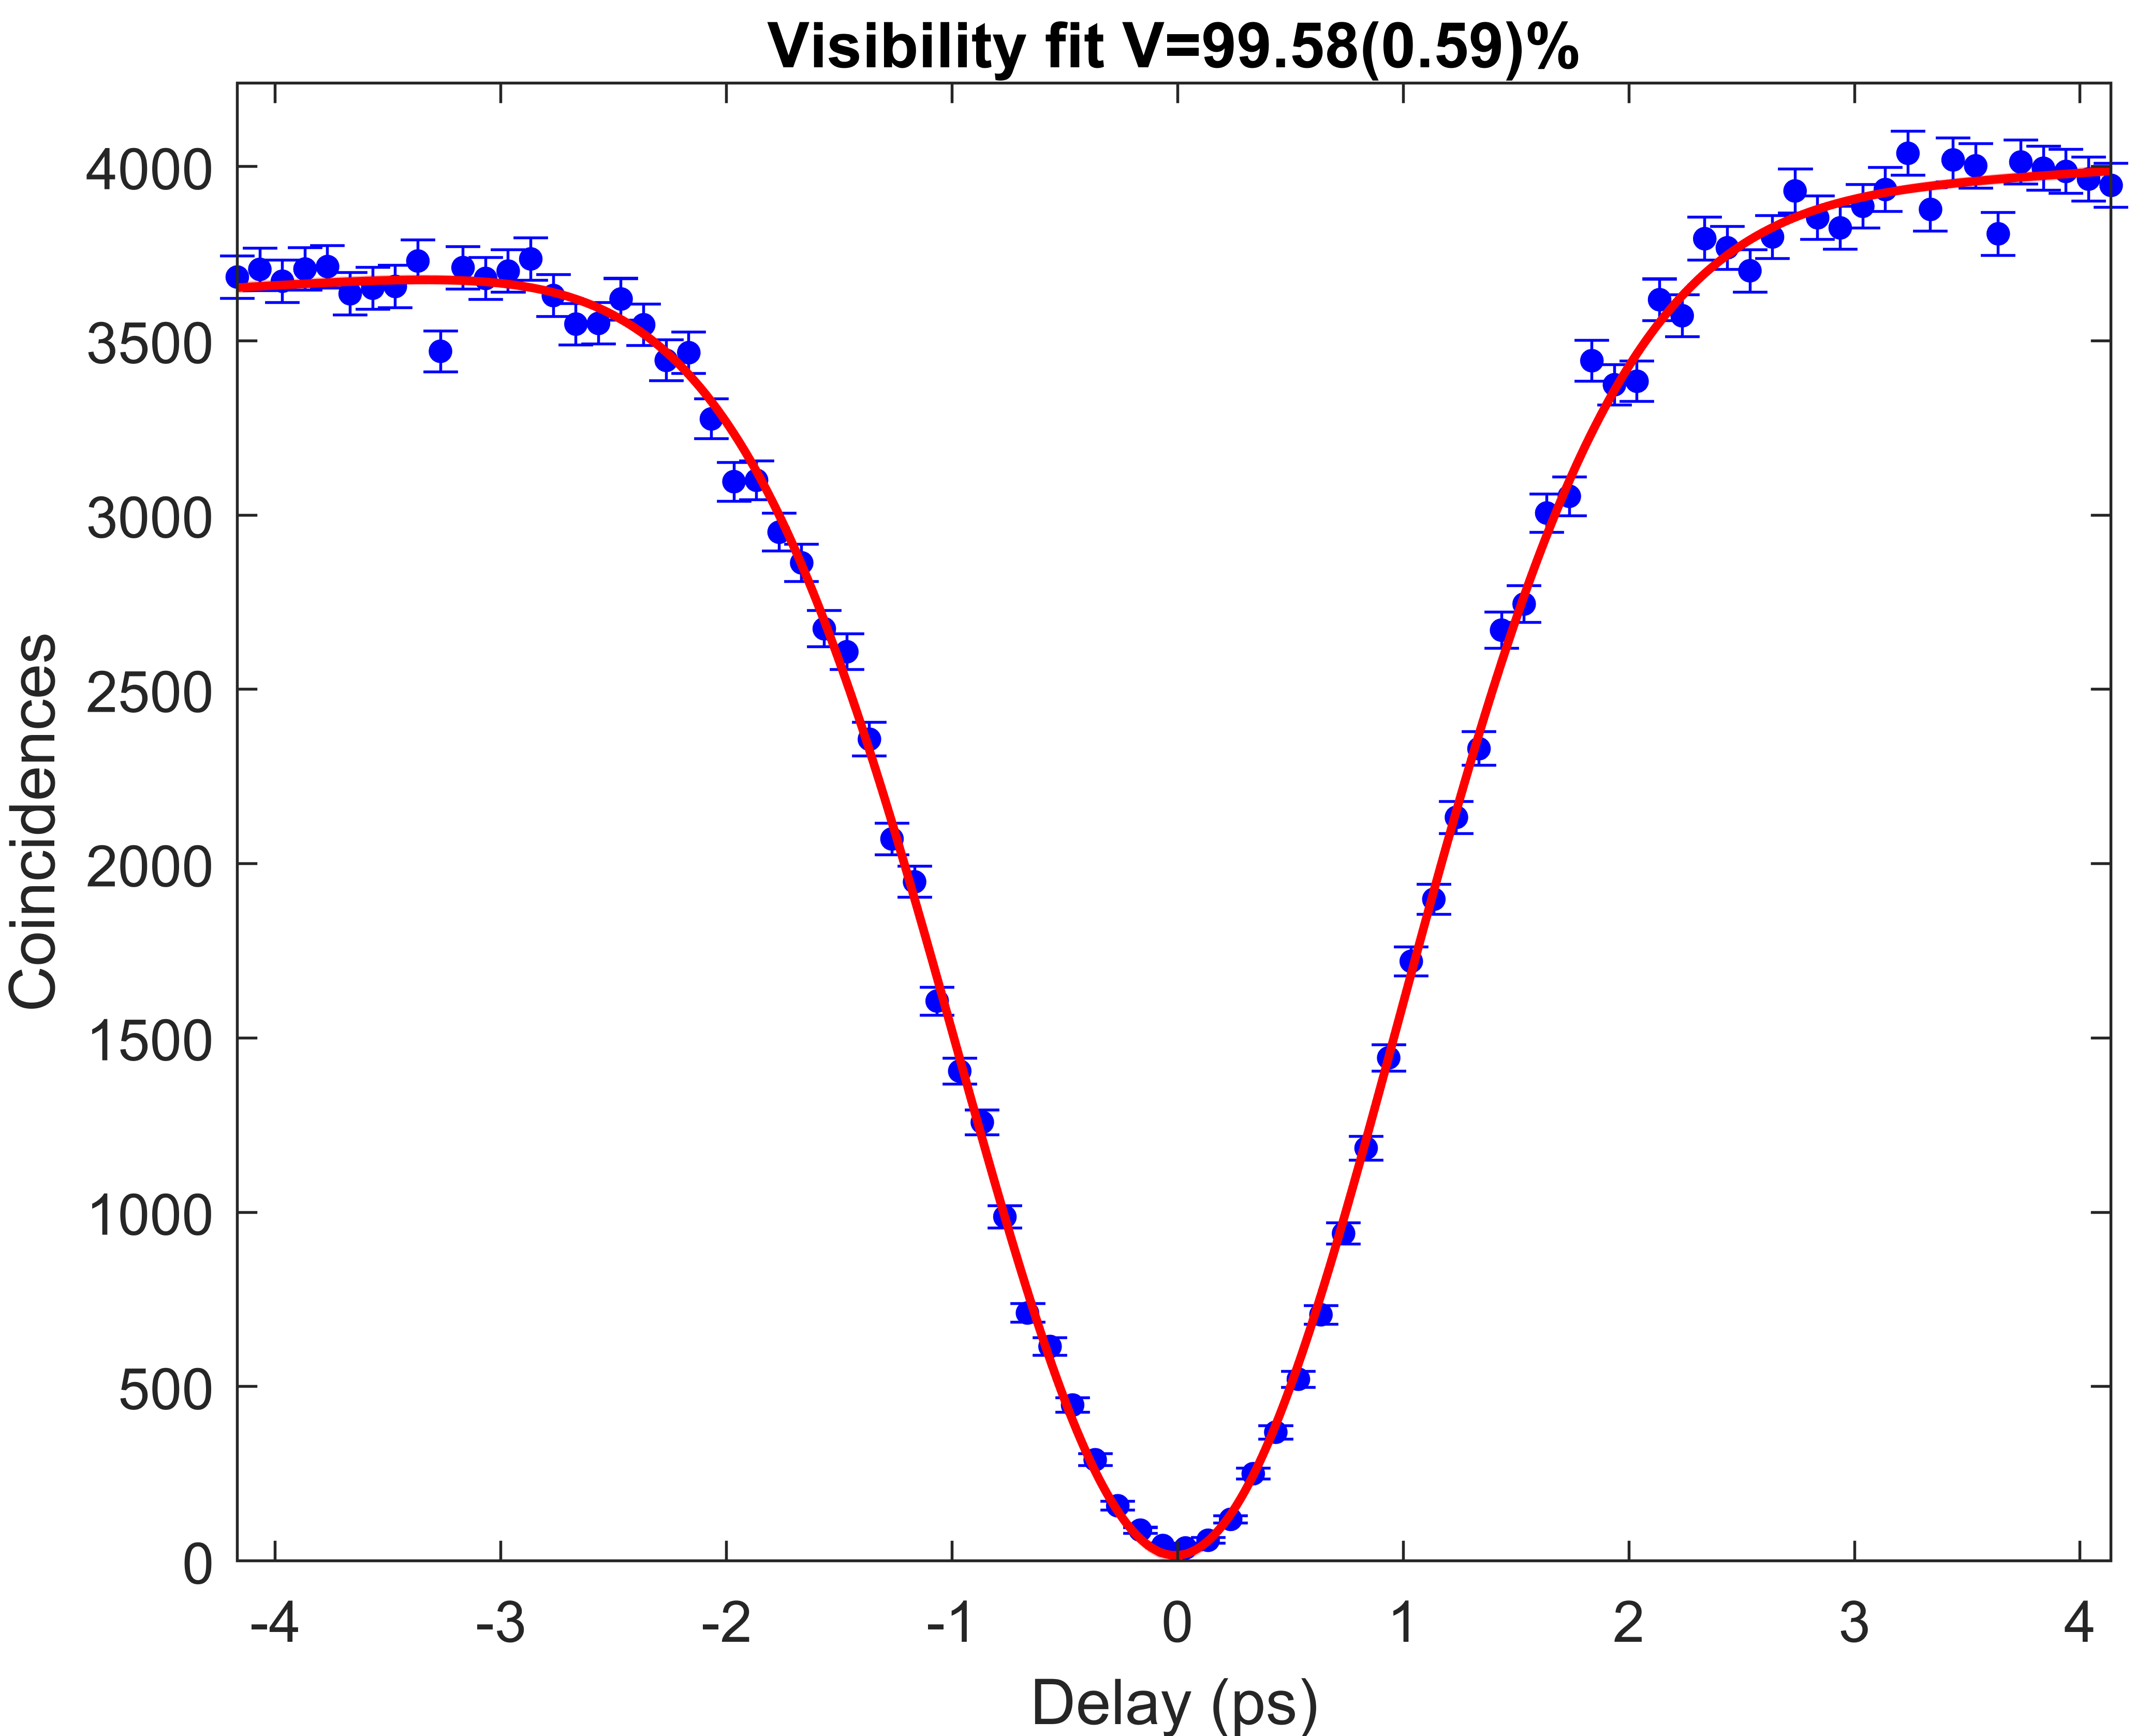
\includegraphics[width=0.8\textwidth]{pics/coincidences_time.png}
        \end{center}
    \end{minipage}    
}

    \block{r}{Spontaneous parametric down-conversion (SPDC) and phase-matching engineering}{
    In SPDC, the down-conversion of a pump photon into two photons is a nonlinear process mediated by the second-order susceptibility $\chi^{(2)}$ of the material when energy and momentum are conserved:\\[0.5cm]
    \raisebox{2ex}{
    \begin{minipage}[b]{0.5\textwidth}
        \centering
        Energy and momentum conservation\\[0.5cm]
        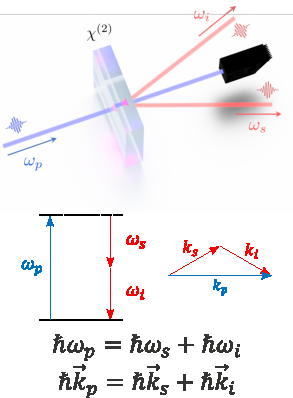
\includegraphics[width=.675\textwidth]{pics/SPDC_scheme_v2.pdf}
    \end{minipage}
    }
    \begin{minipage}[b]{0.5\textwidth}
        \centering
        Quasi-phase matching\\[0.1cm]
        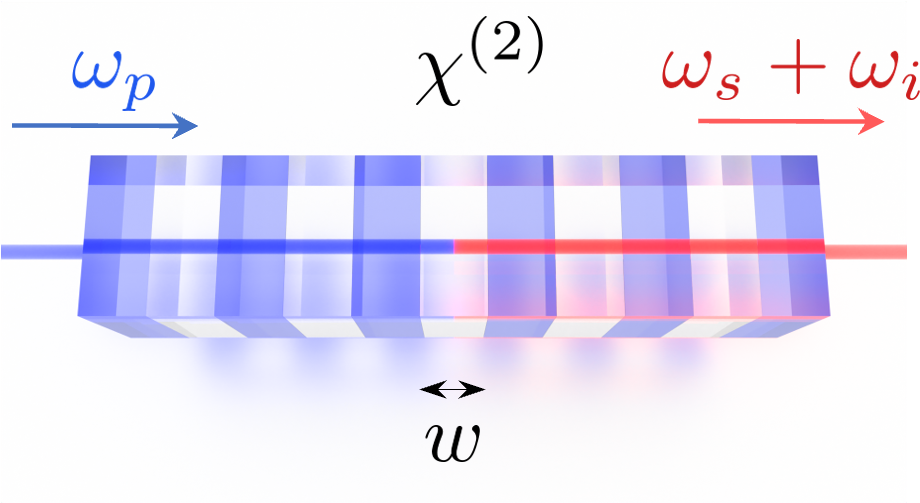
\includegraphics[width=.675\textwidth]{pics/ppKTP.png}\\[0.5cm]
        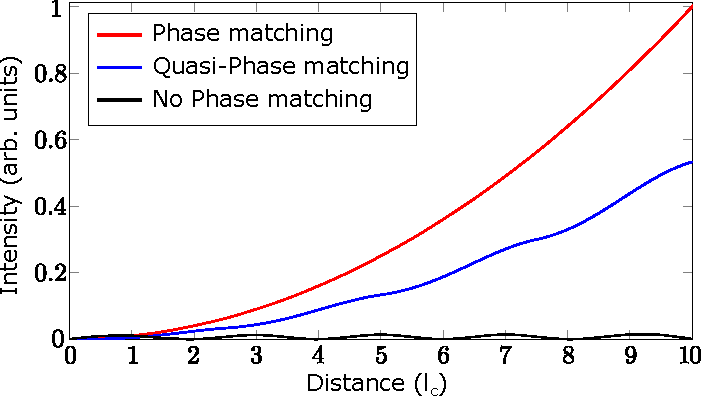
\includegraphics[width=.9\textwidth]{pics/ppKTP_interference.pdf}        
    \end{minipage}
    
    %\raisebox{8ex}{
    %\begin{minipage}[b]{0.3\textwidth}
    %    \centering
    %    Sagnac configuration$^{8,9}$\\[4cm]
    %    \includegraphics[width=\textwidth]{pics/SagnacLoop_v2.pdf}
    %\end{minipage}
    %}
    }
    
    \block{l}{Joint Spectral Amplitude (JSA) engineering}{
        The bi-photon wave function $\ket{\psi}_{s,i}=\iint \mathrm{d}\omega_s \mathrm{d}\omega_i f(\omega_s,\omega_i) \hat{a}^{\dagger}_s(\omega_s)\hat{a}^{\dagger}_i(\omega_i)\ket{0}$ depends on the JSA $f(\omega_s,\omega_i)=\phi(\omega_s,\omega_i)\alpha(\omega_s+\omega_i)$. This directly relates to energy and momentum conservation:\\[0.25cm]
        \begin{itemize}
            \item energy conservation $\Rightarrow$ Pump envelope function $\alpha(\omega_p)=\alpha(\omega_s + \omega_i)$
            \item momentum conservation $\Rightarrow$ Phase-matching function $\phi(\omega_s, \omega_i)=\int \chi^{(2)}(z)e^{i\Delta k(\omega_i,\omega_s)z}\mathrm{d}z$
        \end{itemize}
        \phantom{space}\\[0.2cm]
        \textbf{JSA of a periodically-poled crystal and  Gaussian envelope function:}\\[0.25cm]
        {\centering
        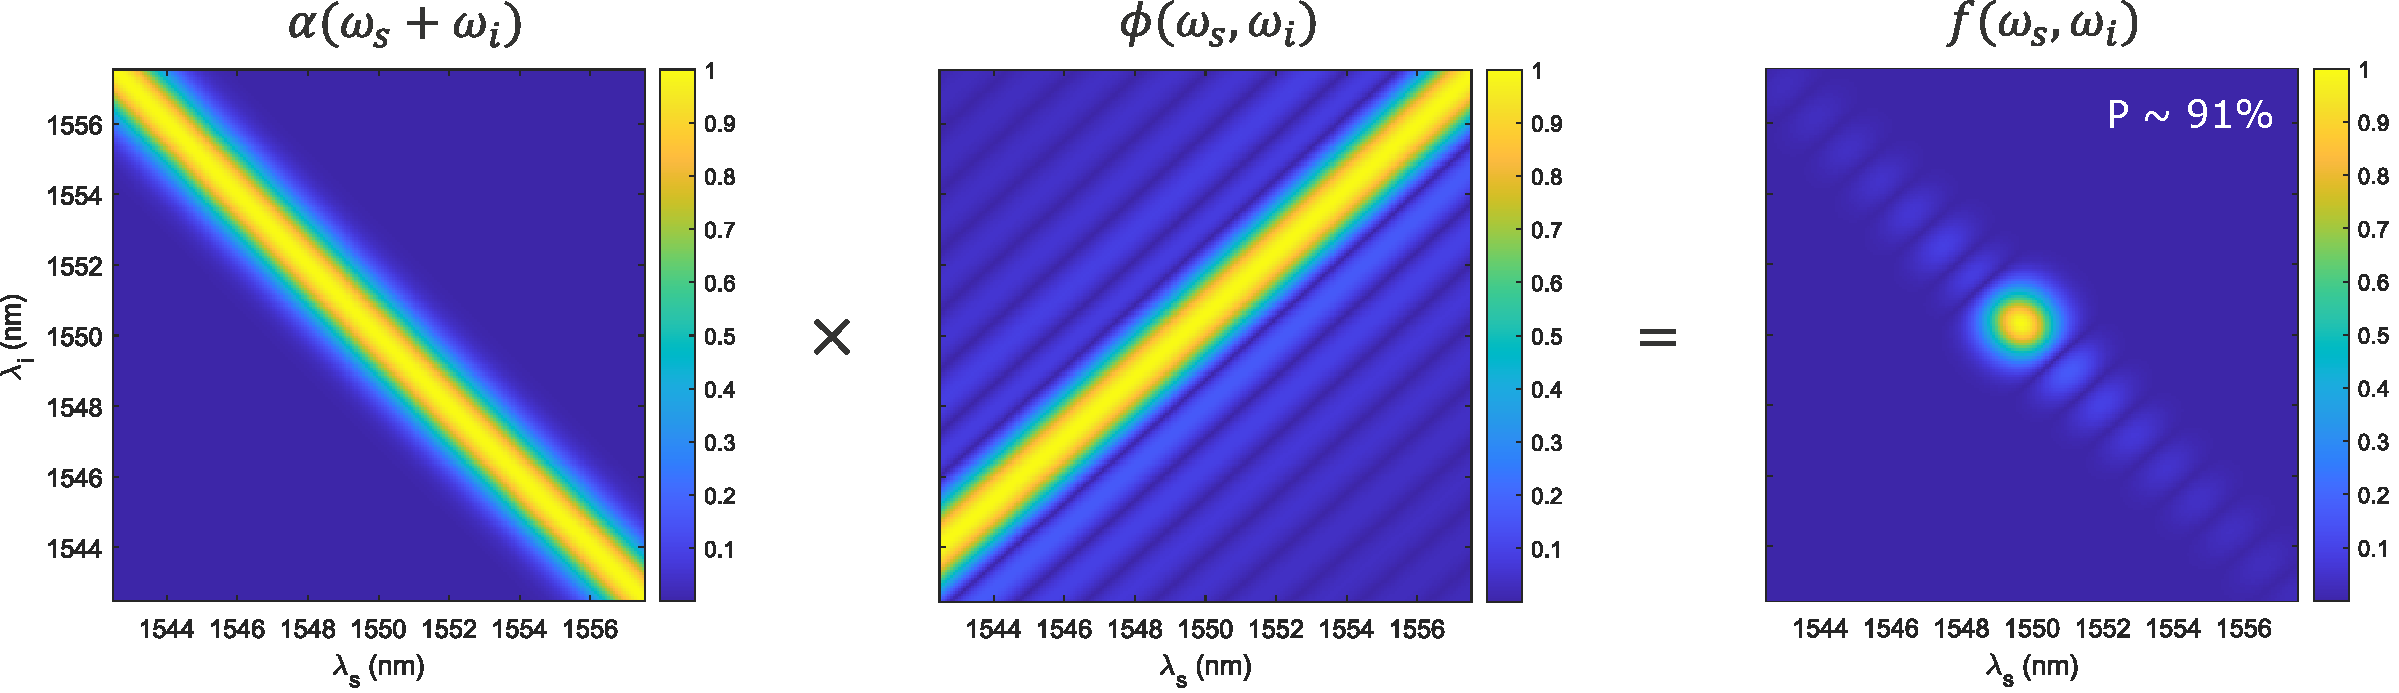
\includegraphics[width=\textwidth]{pics/JSA_ppKTP.pdf}}
        \phantom{space}\\
        \textbf{JSA using a Gaussian phase-matching function and Gaussian envelope function:}\\ [0.25cm]
        {\centering
        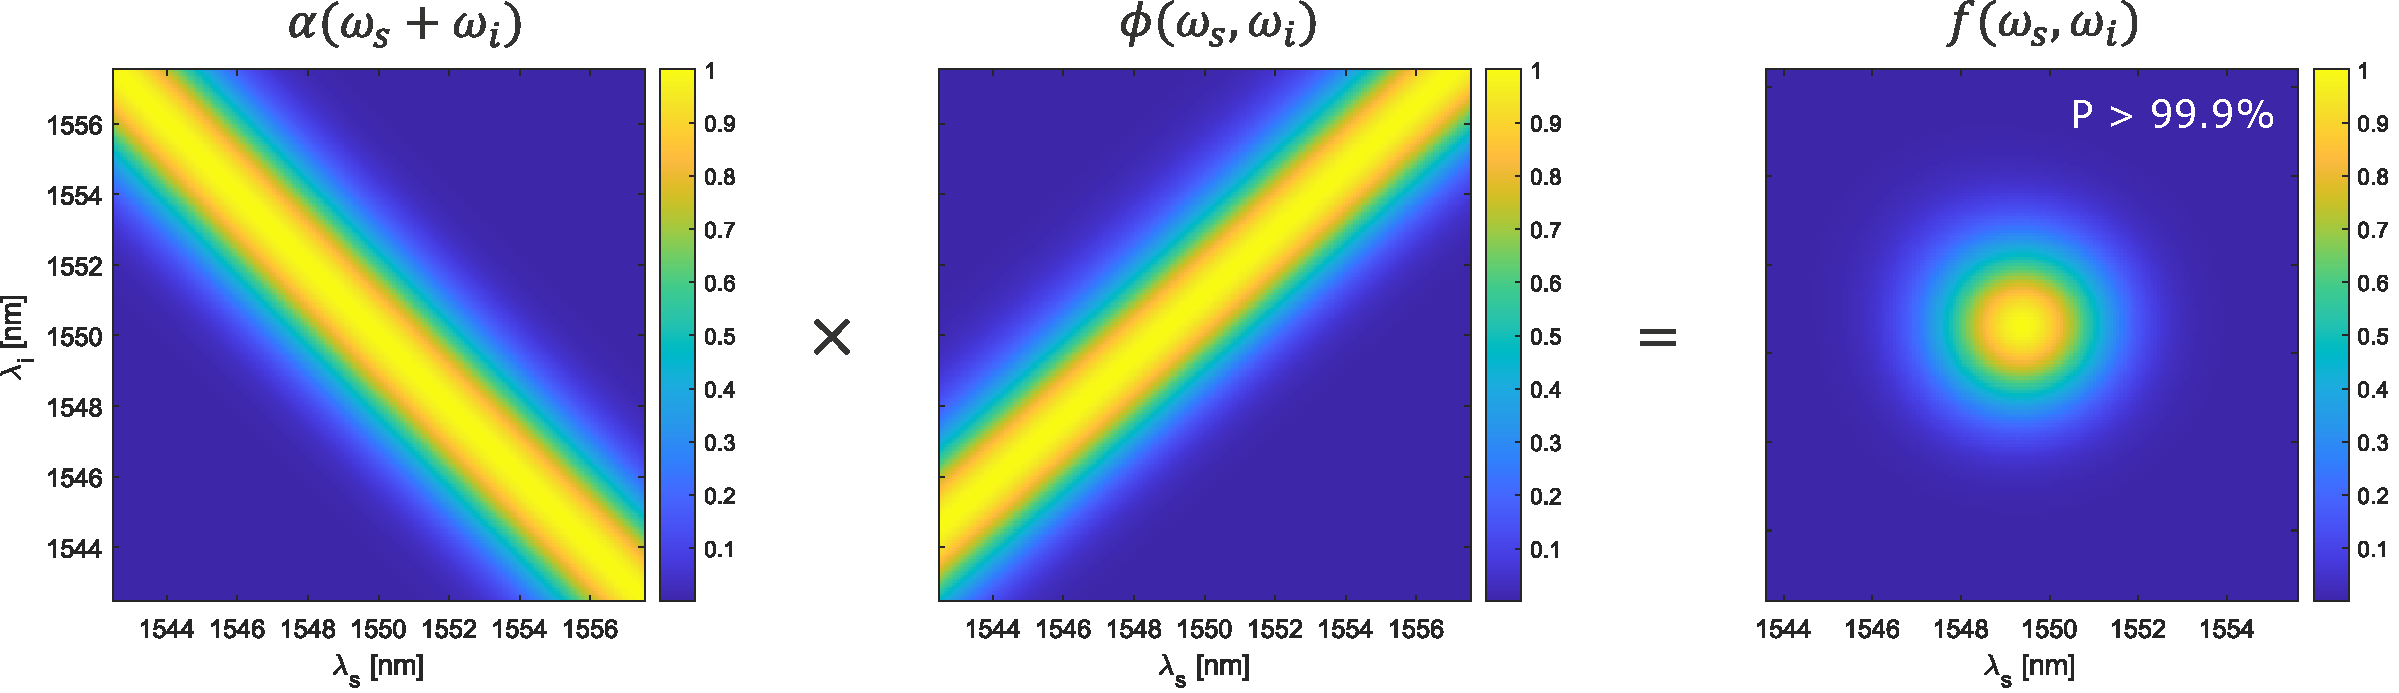
\includegraphics[width=\textwidth]{pics/JSA_aKTP.pdf}}

        Optimal purity is only possible when both the phase-matching function and the pump envelope function are Gaussian with equal width $\sigma$ [3]. This requires simultaneous engineering of the poling of the nonlinear material [4] and spectral shaping of the pump laser:
        
        {\centering
        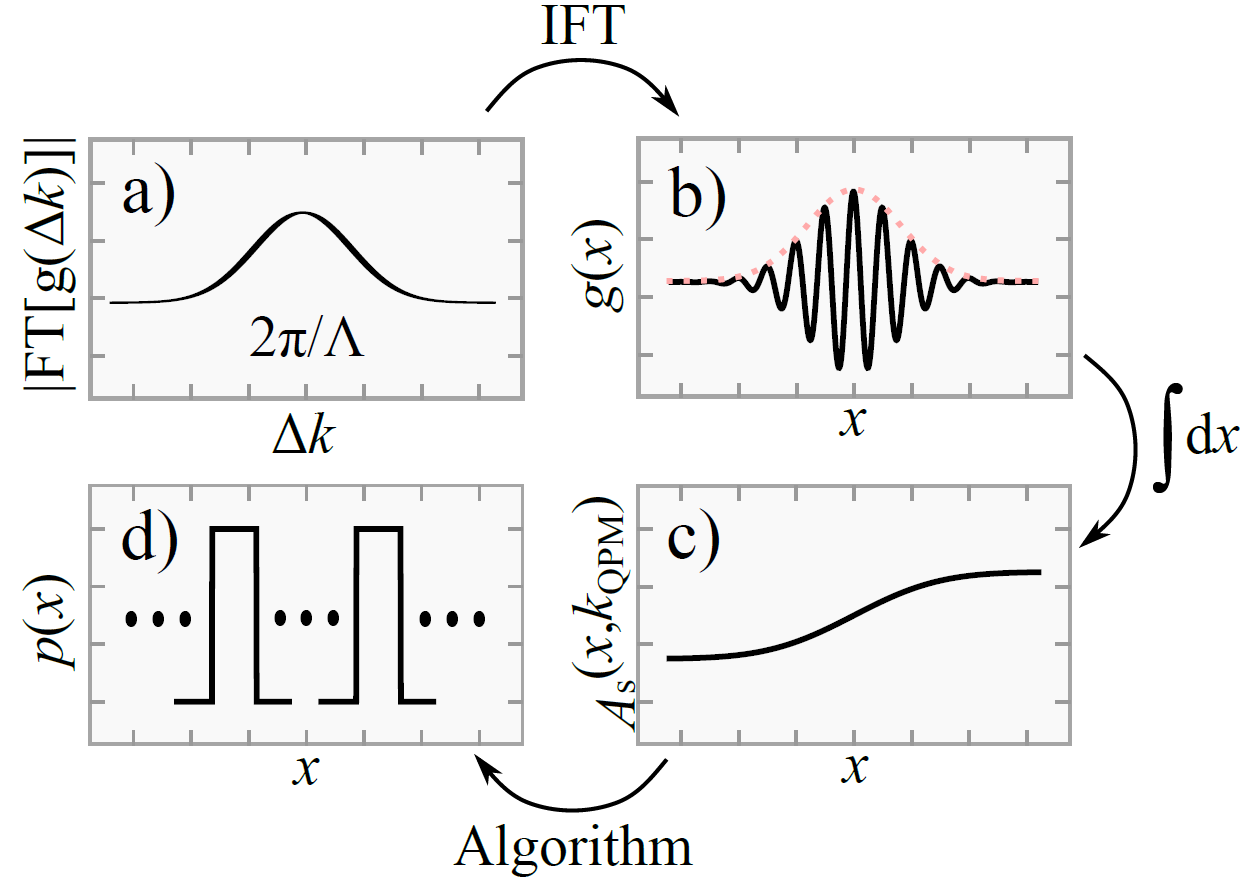
\includegraphics[width=0.4\textwidth]{pics/TambascoProcedure.png}}
        $\,$
        {\centering
        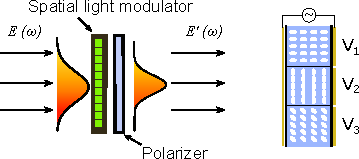
\includegraphics[width=0.55\textwidth]{pics/SLM_scheme.pdf}}
    }

    \block{r}{Experimental setup and results}{
    {\centering
    \includegraphics[width=0.99\textwidth]{pics/Setup_PureSources_v3.png}}\\[0.25cm]
    
    % Example pump spectral shaping
    \textbf{Pump spectral shaping}\\[0.25cm]
    %The laser is spectrally shaped via an SLM at the Fourier plane of a 4$f$ pulse shaper and pumps two domain-engineered potassium titanyl phosphate (aKTP) crystals. Two down-converted photons are interfered in a heralded four-photon HOM setup and detected with superconductive nanowire single-photon detectors (SNSPDs).
    {\centering
        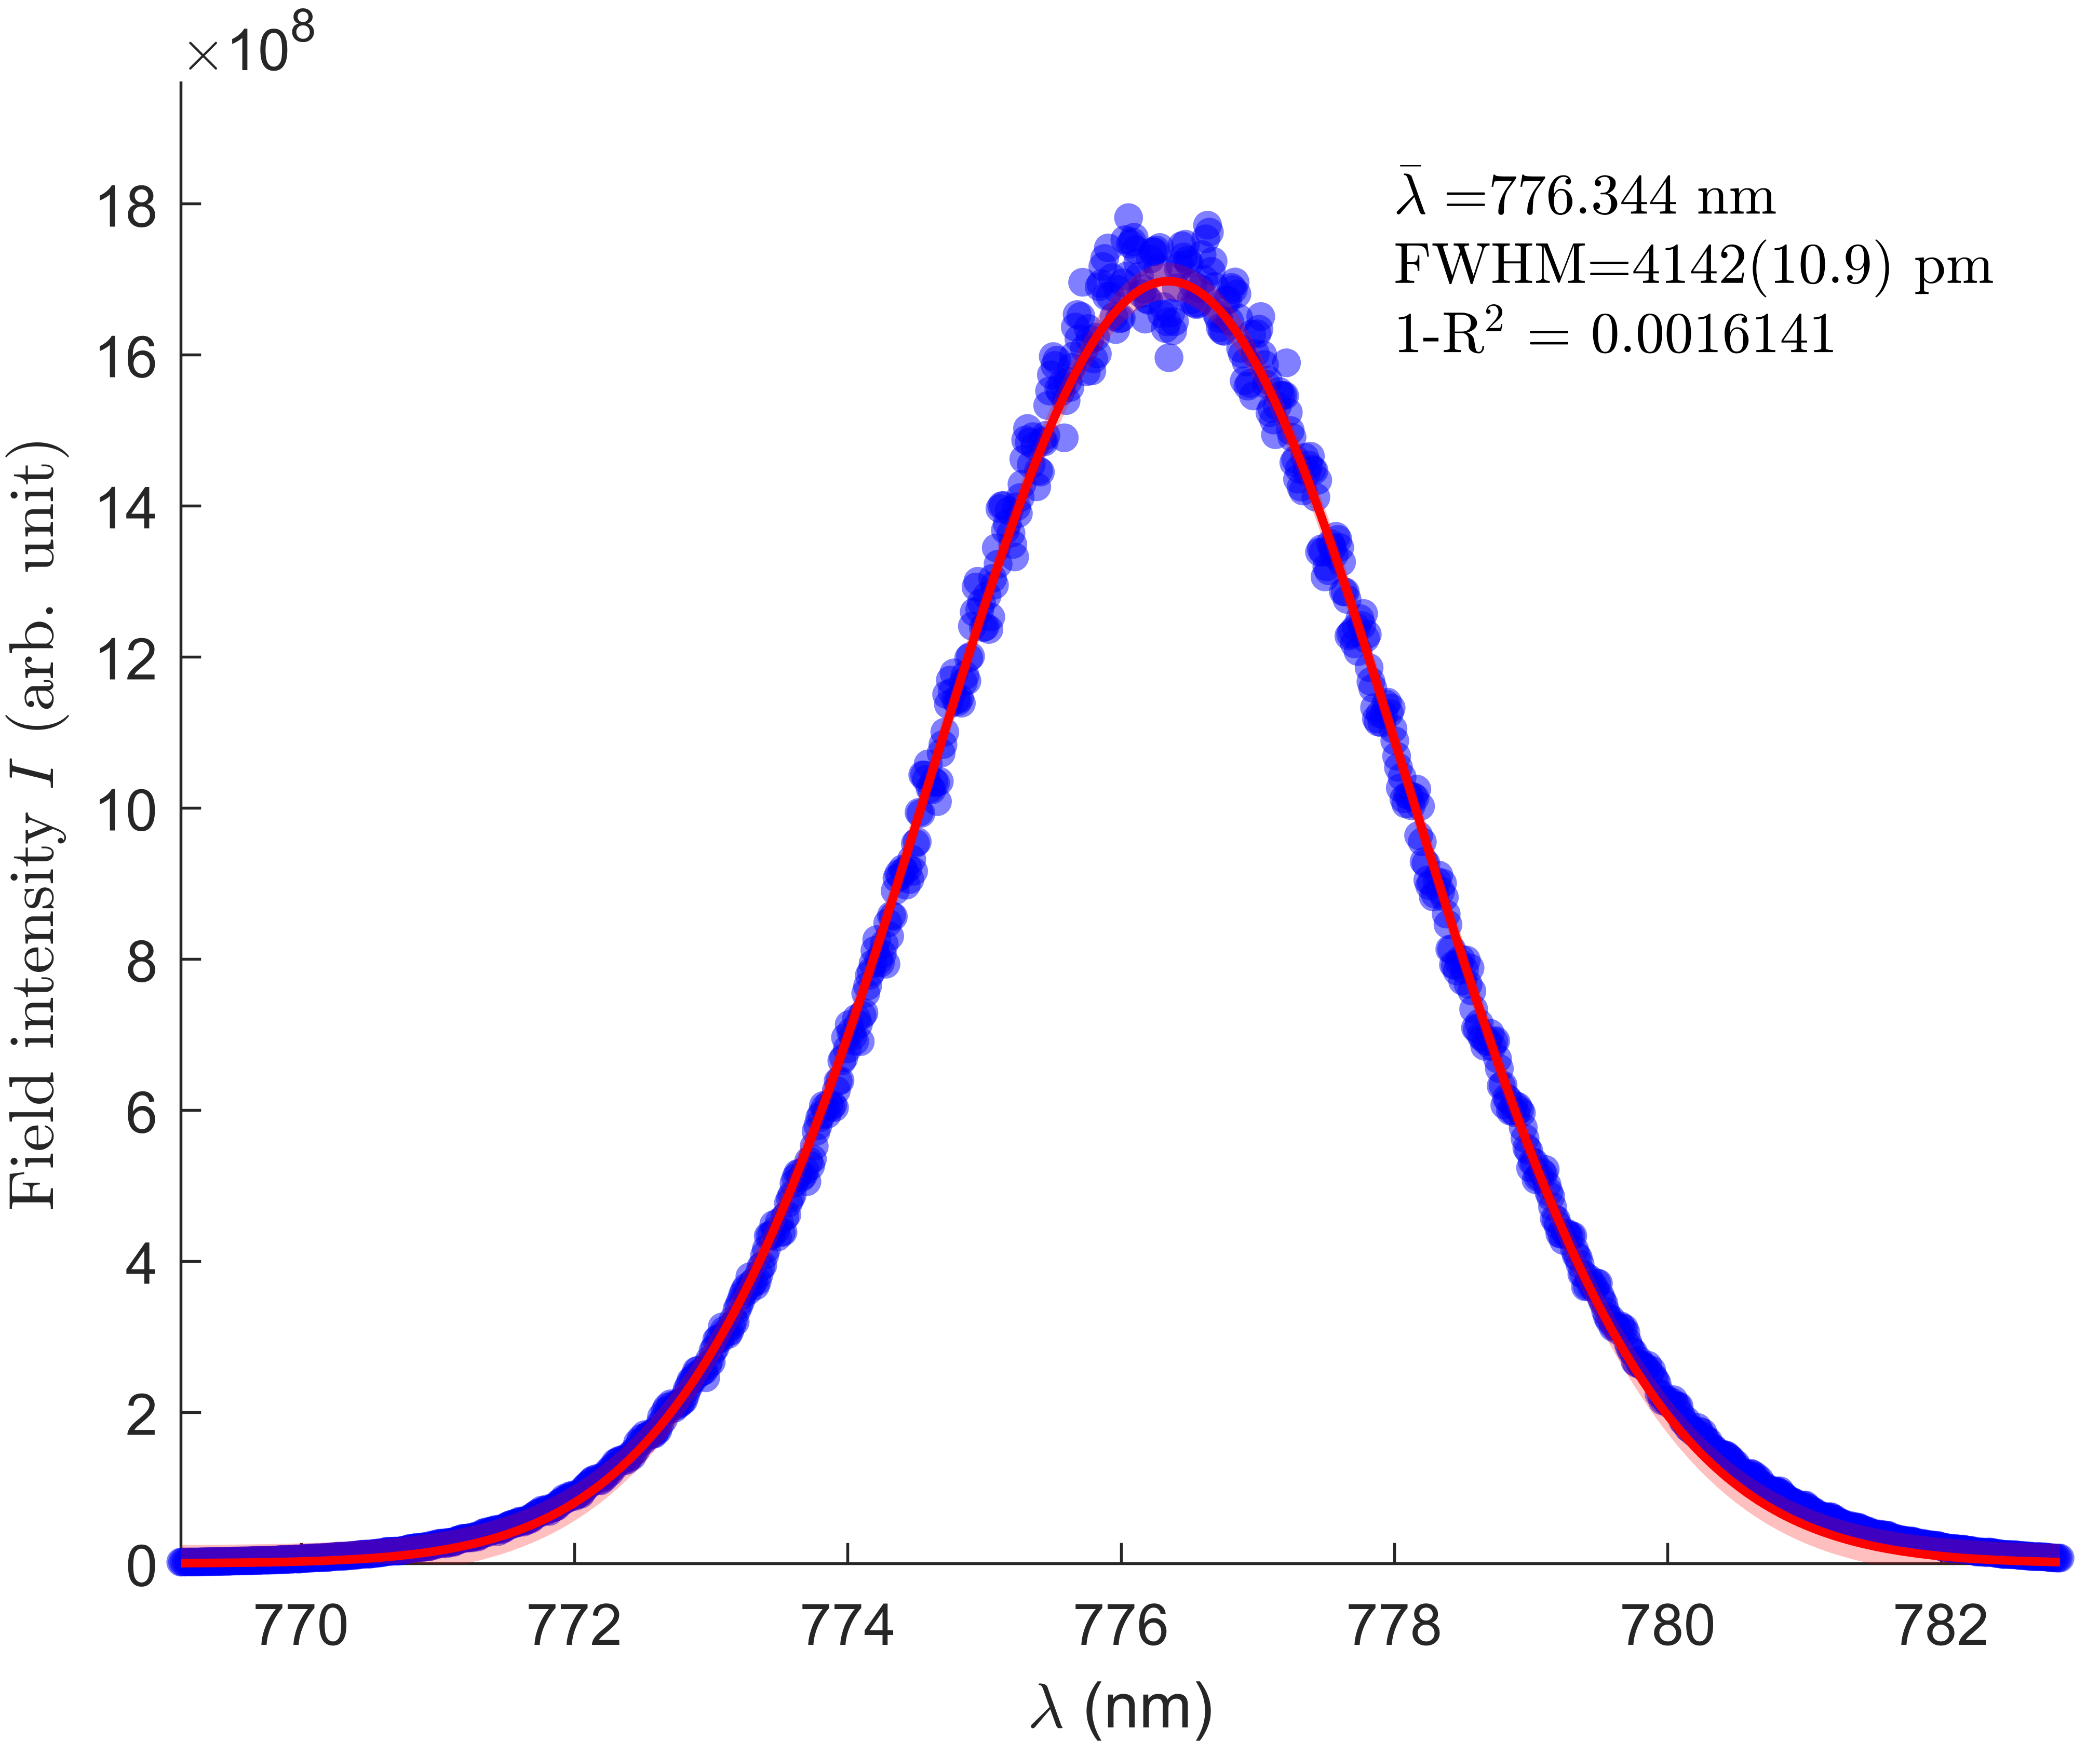
\includegraphics[width=0.3\textwidth]{pics/MiraOutput_intensity.png}}
        {\centering
        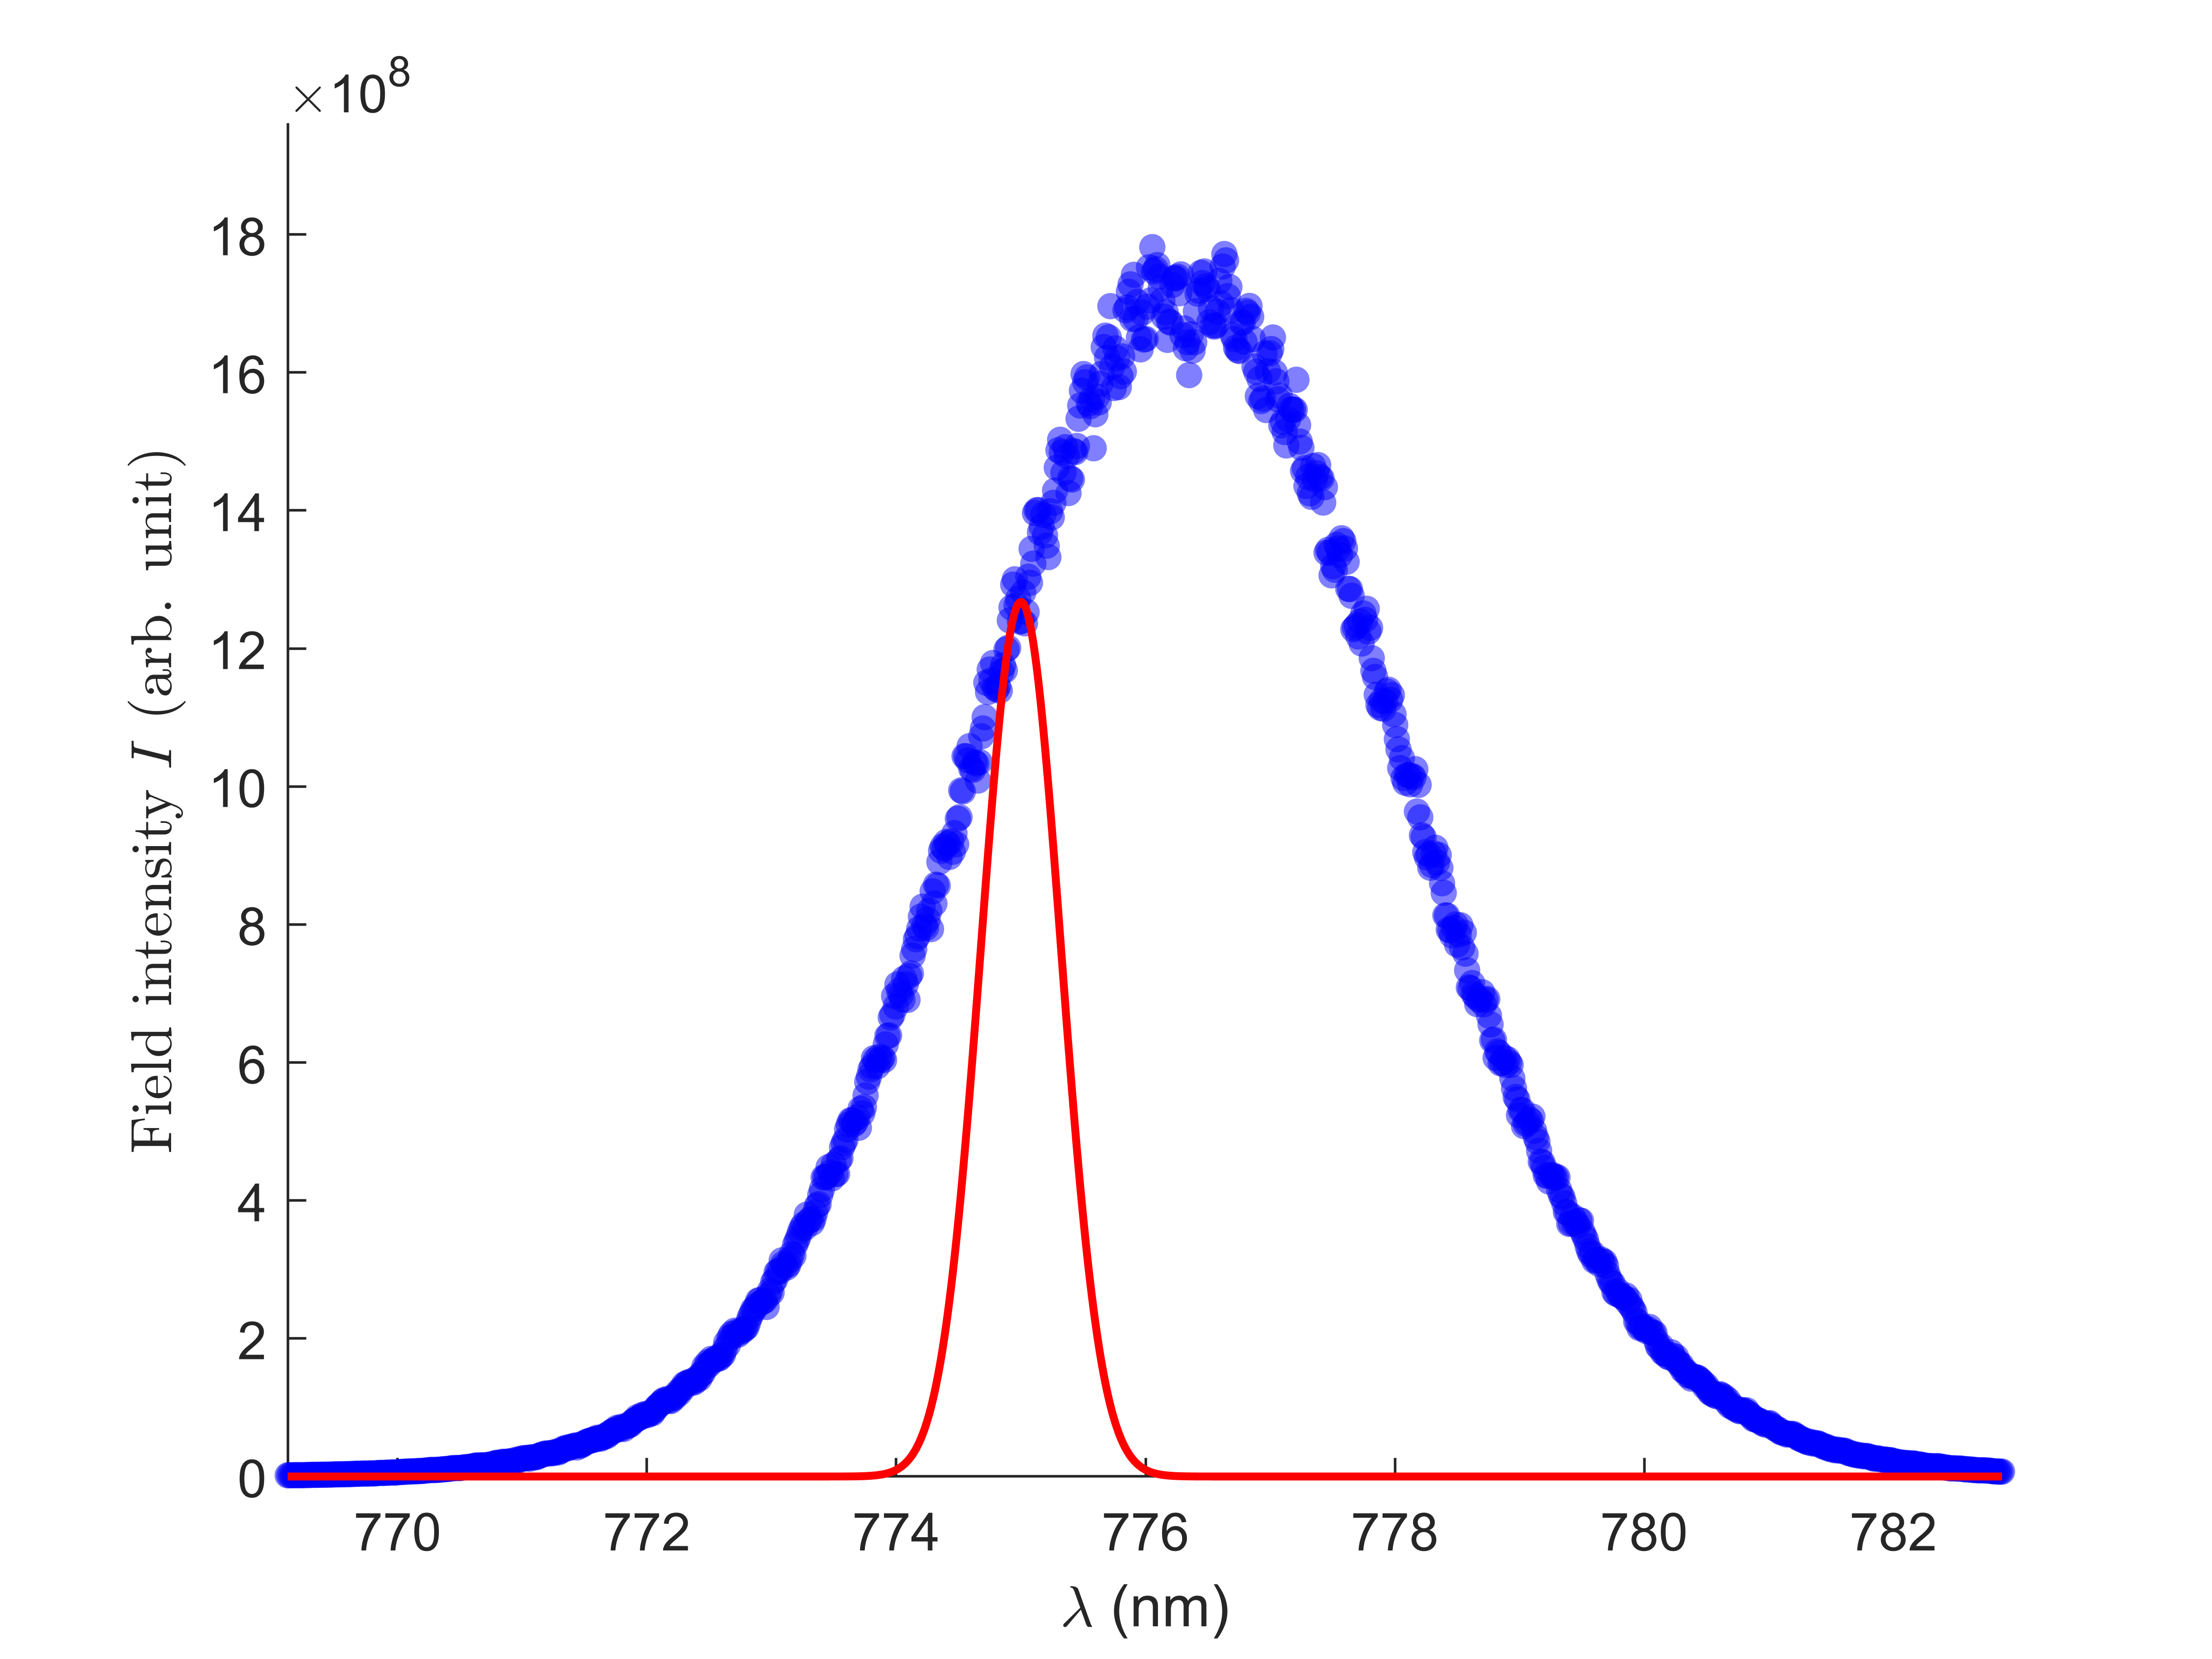
\includegraphics[width=0.34\textwidth]{pics/MiraOutput_intensity_idealGauss.png}}
    {\centering
        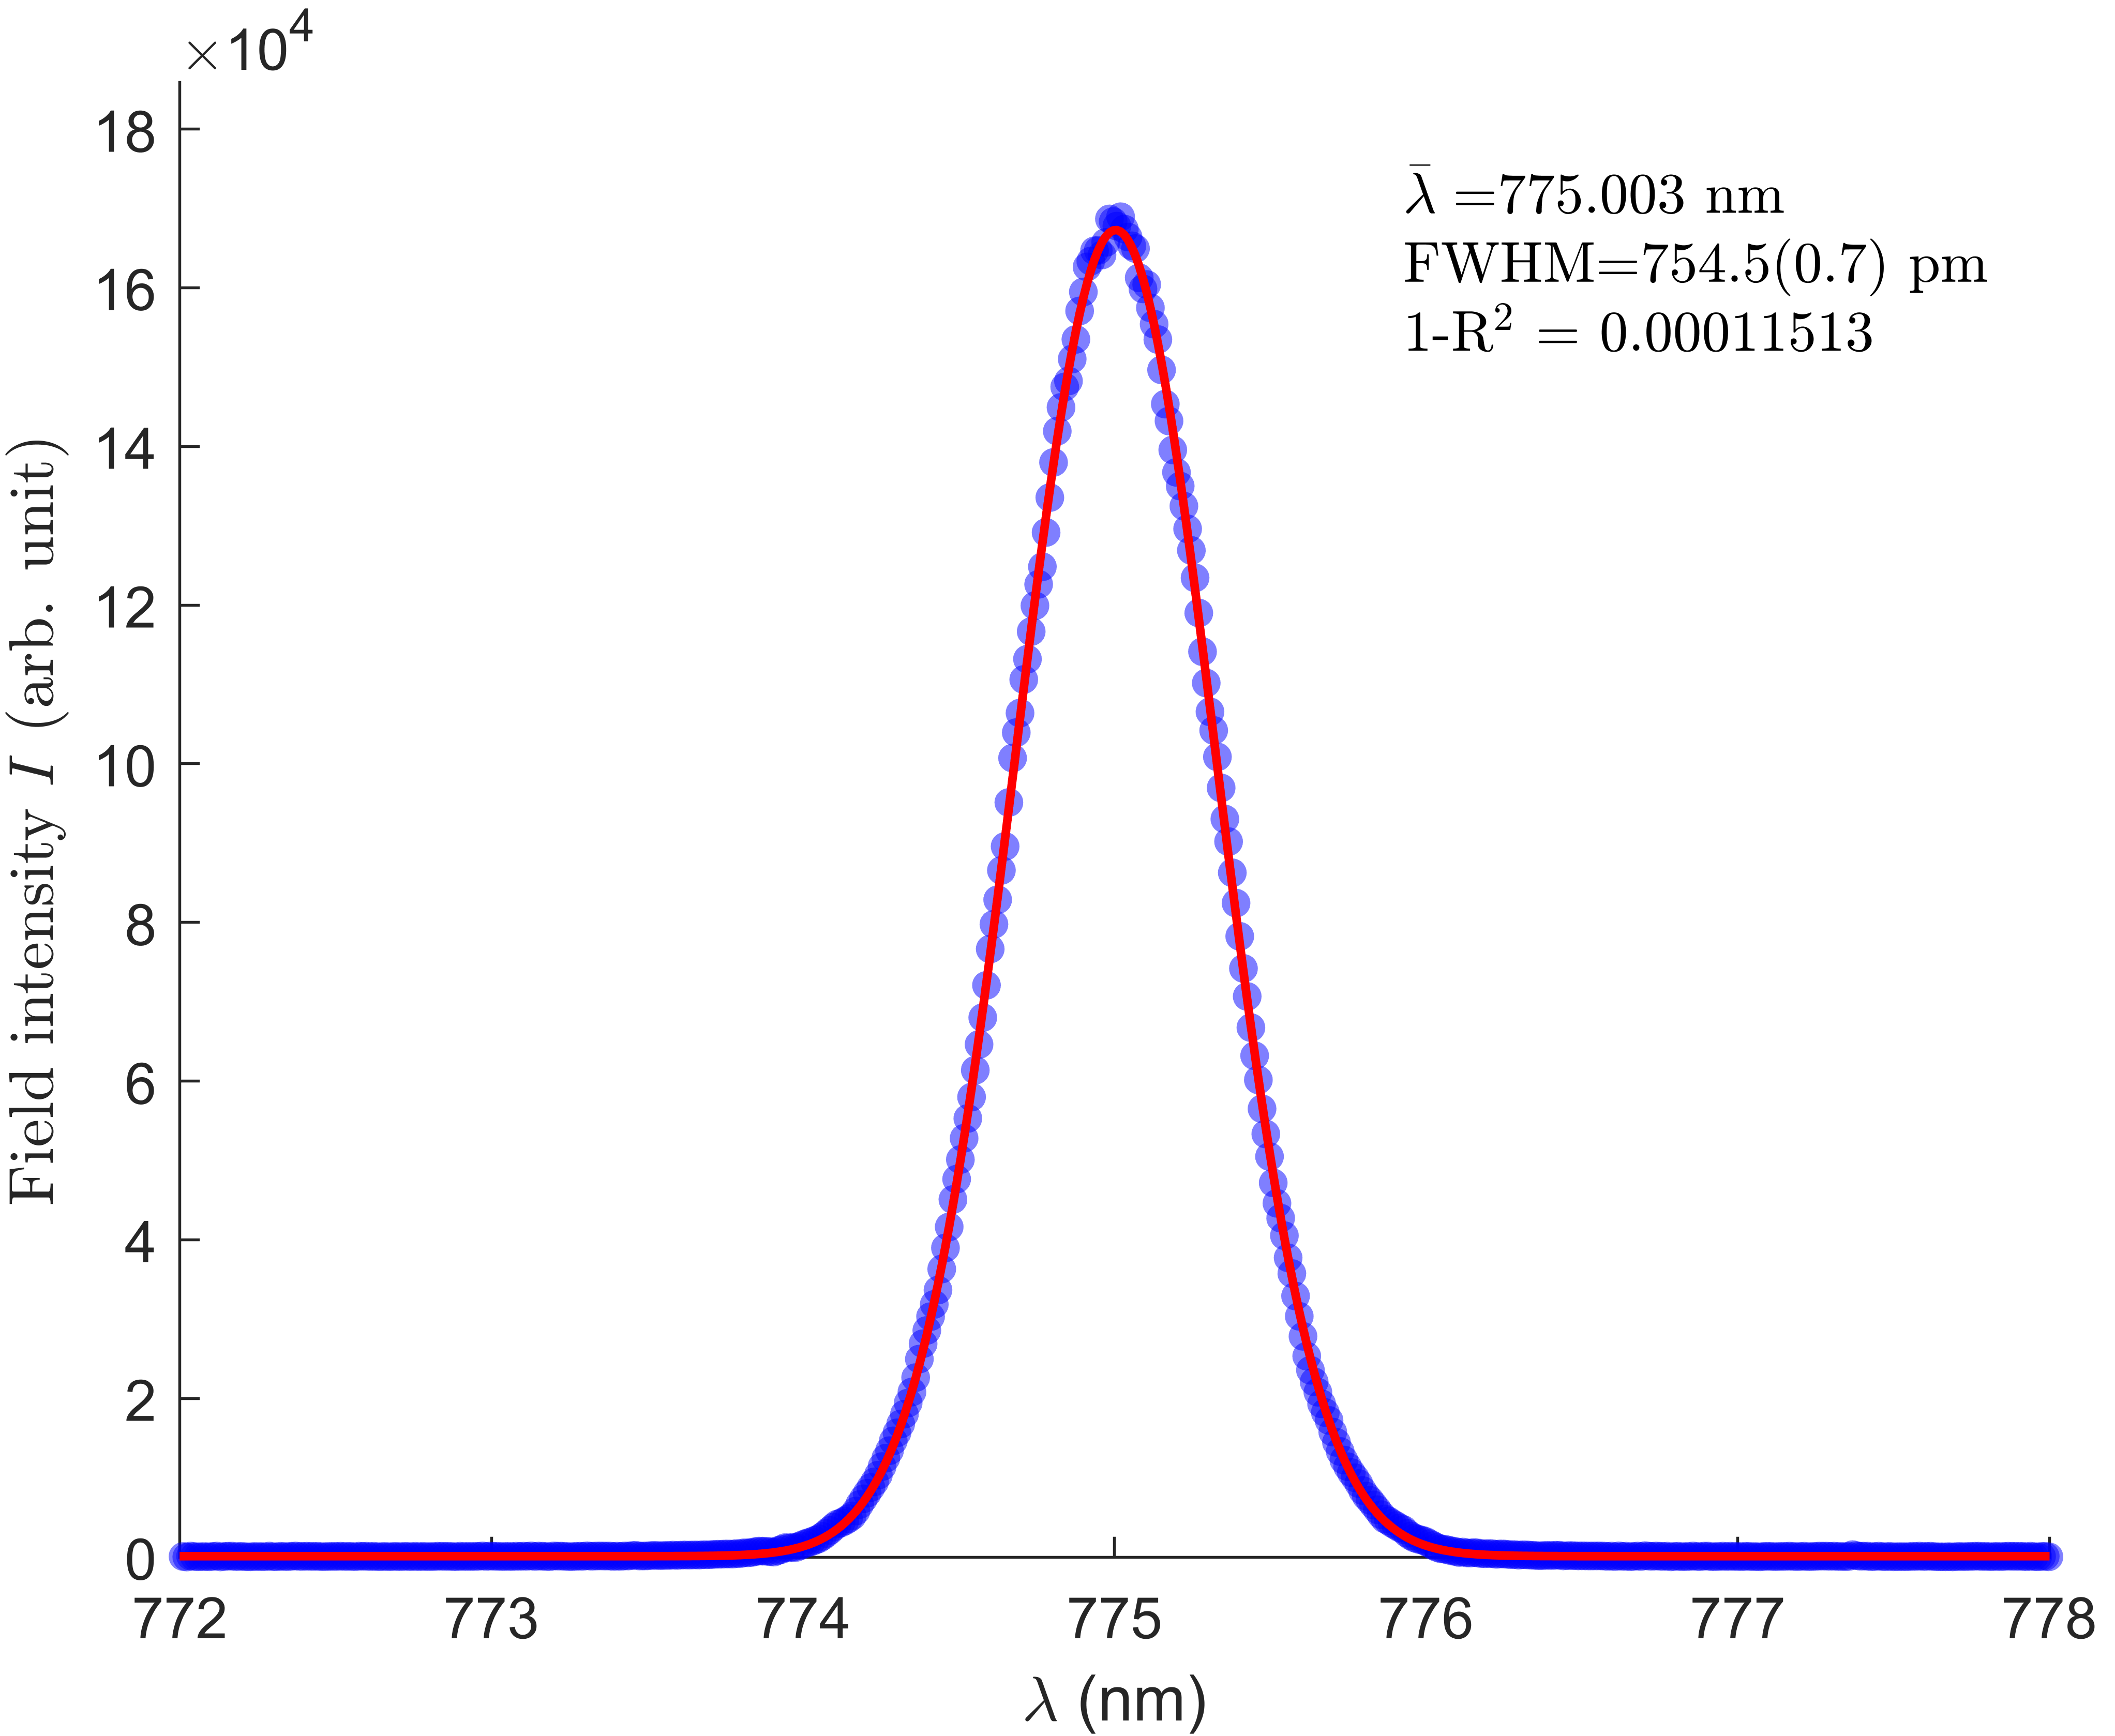
\includegraphics[width=0.3\textwidth]{pics/775.00nm-fwhm0.7411nm-r2_0.9996_intensity.png}}
    \phantom{space}\\[0.25cm]

    % Measurements JSA and HOM
    \textbf{JSA reconstruction and HOM dip measurements}\\[0.25cm]
    % JSA measurement
    \includegraphics[width=0.39\textwidth]{pics/Purity99.82_normJSA.png}
    $\qquad \qquad$
    % HOM measurement
     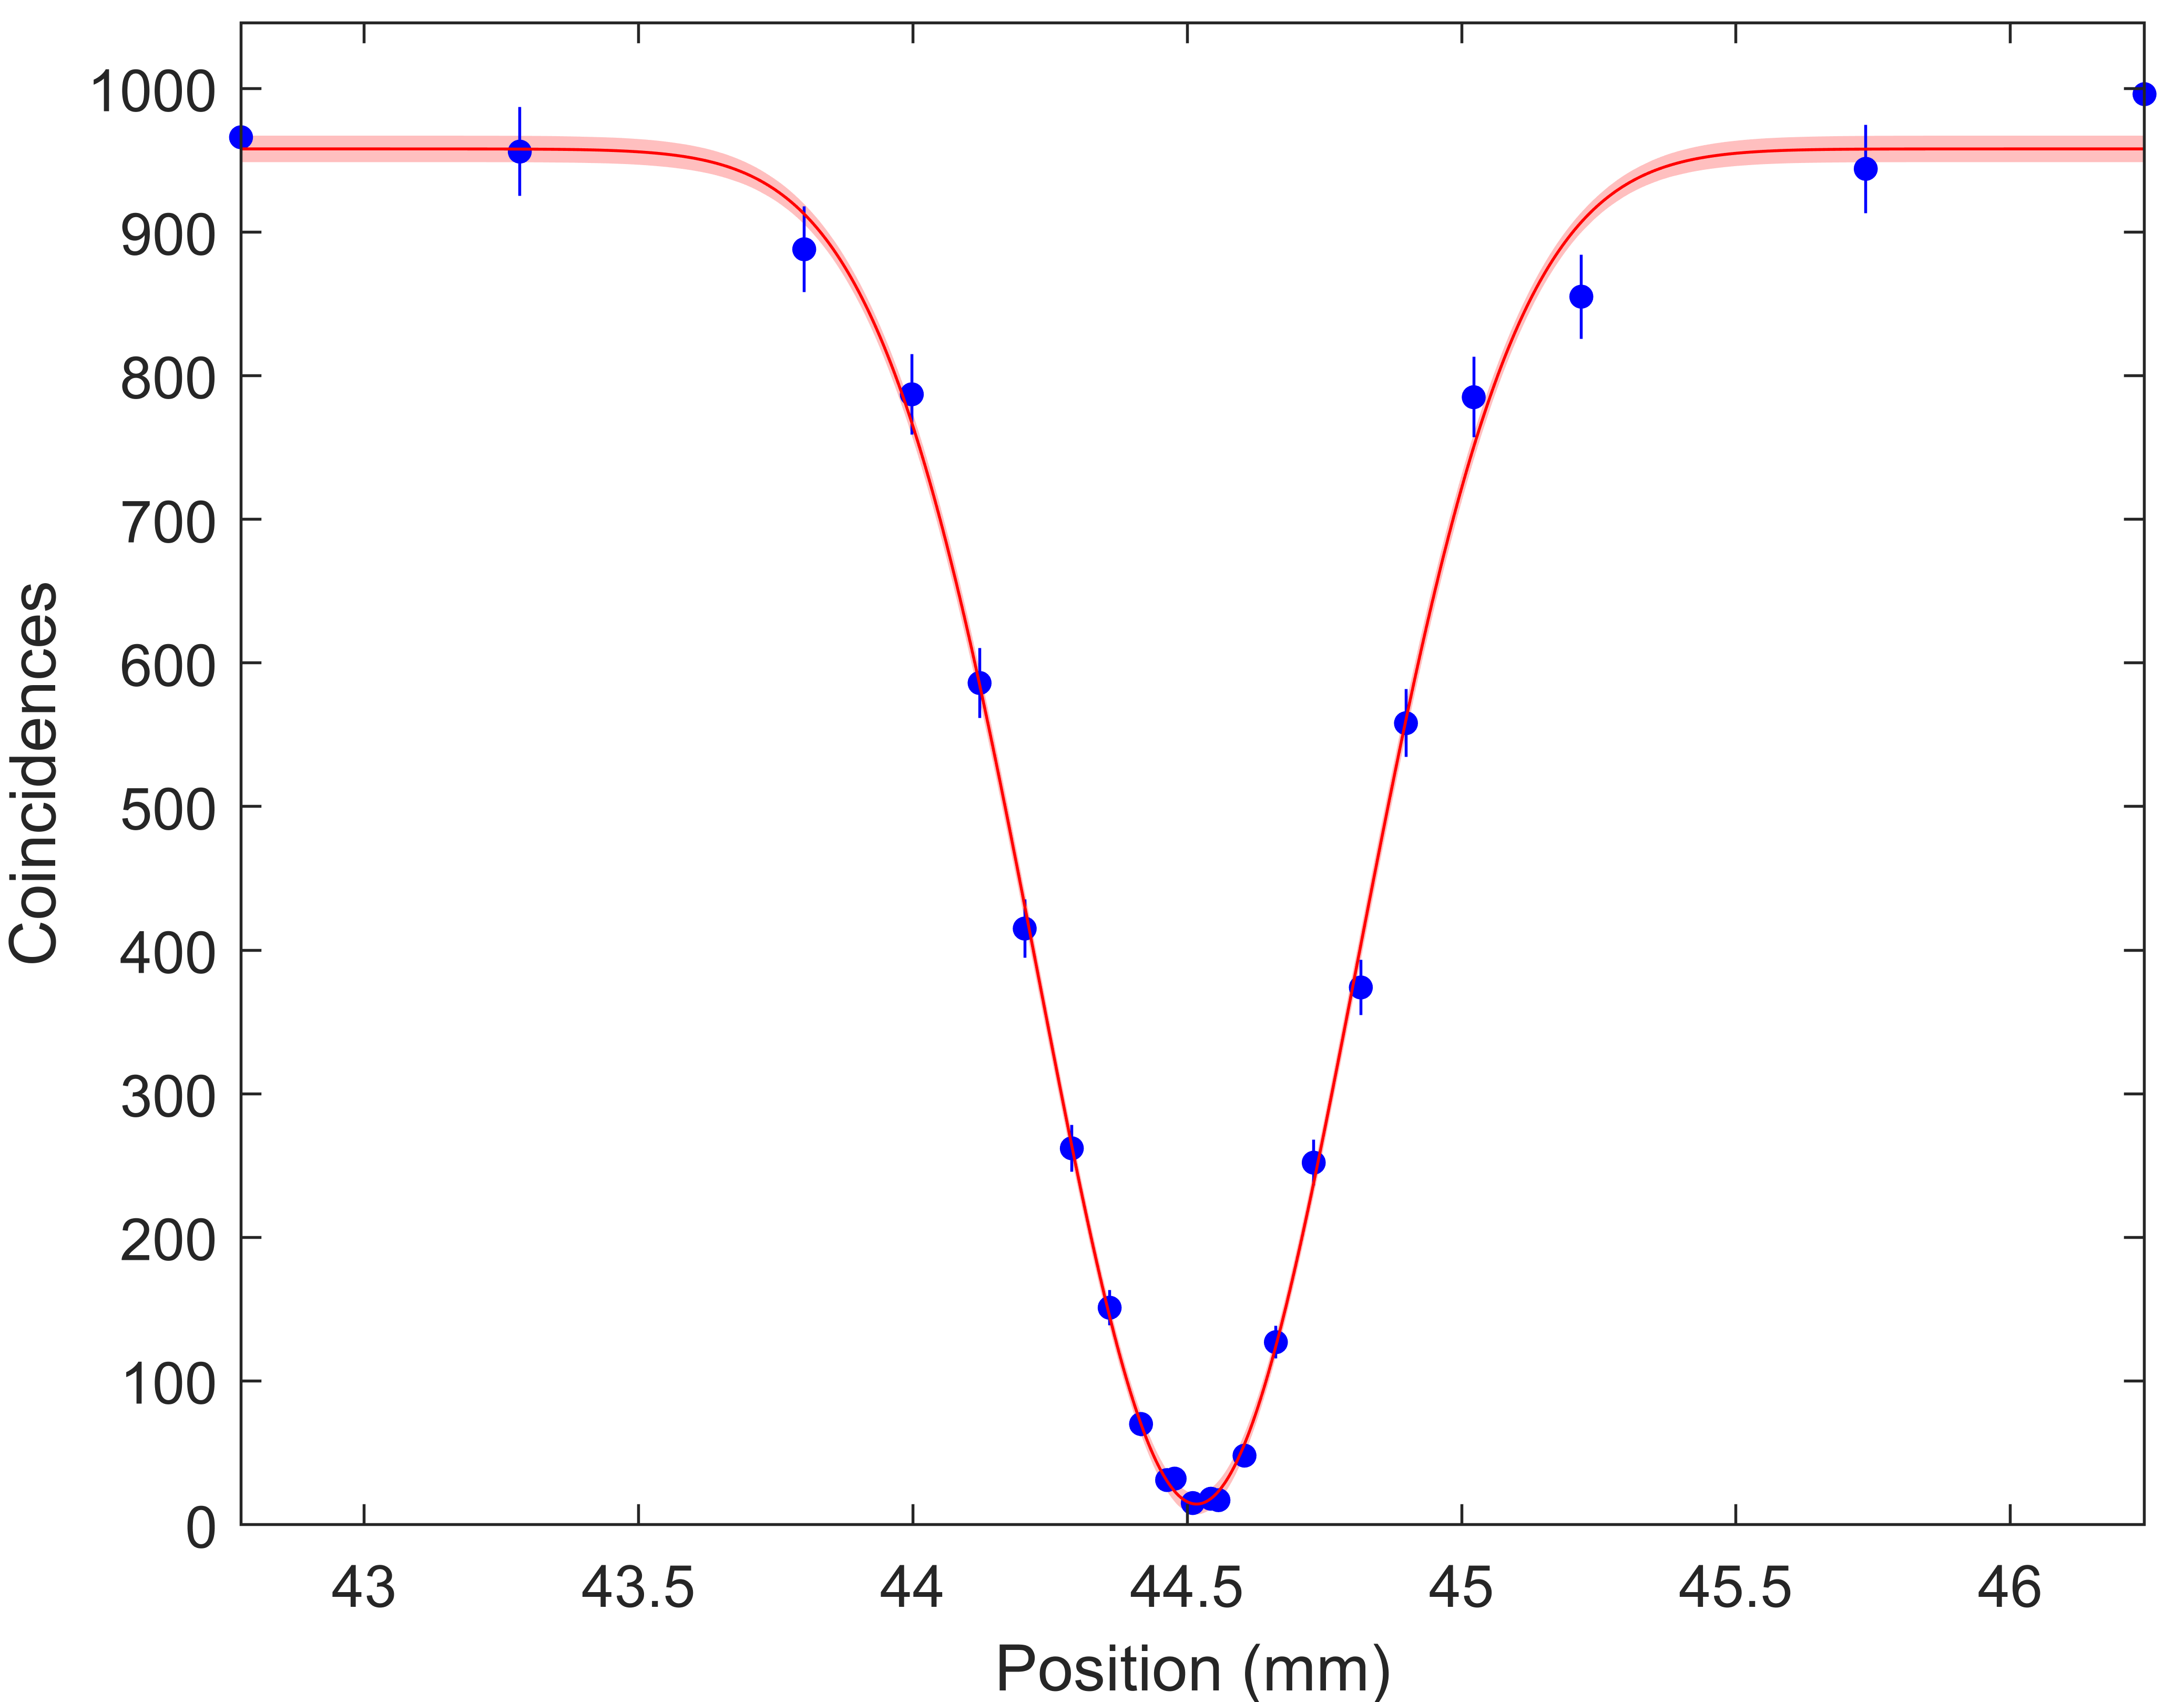
\includegraphics[width=0.42\textwidth]{pics/coincidences_noLabel.png}
     \phantom{space}\\[0.2cm]
    with measured values:
    \begin{itemize}
        \item Spectral purity (via singular value decomposition [4]) $\mathbf{P=99.92(1)\%}$
        \item HOM dip visibility $\mathbf{V_{fit}=98.5(1.5)\%}$ 
    \end{itemize}     
     
}
    
    %\block{l}{Outlook}{
    %}

    \block{l}{References}{
    %\LARGE
    \textbf{[1]} A. Pickston et al., Opt. Express \textbf{29}, 6991-7002 (2021);
    \textbf{[2]} C. K. Hong et al., Phys. Rev. Lett. \textbf{59}, 2044 (1987);
    \textbf{[3]} N. Quesada et al., Phys. Rev. A \textbf{98}, 043813 (2018);
    \textbf{[4]} J-L. Tambasco et al., Opt. Express \textbf{24}, 19616-19626 (2016);
    \textbf{[5]} M. Avenhaus et al., Opt. Lett. \textbf{34}, 2873-2875 (2009);
    \textbf{[6]} P. J. Mosley et al., Phys. Rev. Lett. \textbf{100}, 133601 (2008).
    }
 


\end{poster}
\end{document}

%%% Local Variables:
%%% mode: latex
%%% TeX-master: t
%%% End:
